\section{Boltzmann Machines}\label{sec:bm}
Boltzmann machines are stochastic recurrent neural networks.

Boltzmann machines work similar to Hopfield nets. They have a binary state vector ($x_j \in {0,1}$), but the new state a neuron $x_j$ is determined stochastically (based on the total input $z_j$) on each update of $x_j$.

\begin{equation}
z_j = b_j + \sum_i x_i w_{ij}
\end{equation}
The probability that the activation of neuron $x_j$ is set to $1$ is calculated using the sigmoid function,
\begin{equation}
p(x_j = 1) = \sigma(z_j) = \frac{1}{1 + e^{-z_j}}
\end{equation}
, otherwise the activation of $x_j$ becomes $0$.

In general Boltzmann machines are unrestricted (see \ref{sec:rbm} for \gls{RBM}), but have the properties:
\begin{itemize}
\item Network is fully connected
\item No self connections, $w_{ii}=0$
\item Undirected/symmetric, $w_{ij}=w_{ji}$
\end{itemize}

One can define input neurons that have the fixed input value during evaluation.

\subsection{Energy}
The energy of a state $x$ is defined by
\begin{equation}
E(x) = - \sum_i x_i b_i - \half \sum_{i<j} x_i x_j w_{ij}
\end{equation}

With this we can calculate the probability of a state $x$
\begin{equation}
p(x) = \frac{e^{-E(x)}}{\sum_y e^{-E(y)}}
\end{equation}

In average updating the neurons will decrease the energy in the network.

\subsection{Simulated Annealing}
Use temperature $T$ to allow more changes in the beginning (\eg jumps out of bad local minima) by using the sigmoid function with $\beta=\frac{1}{T}$.
\begin{equation}
p(x_j = 1) = \frac{1}{1 + e^{\frac{-z_j}{T}}}
\end{equation}
Figure \ref{fig:bm-simulated-annealing} shows curves with different temperature.

\begin{figure}
\centering
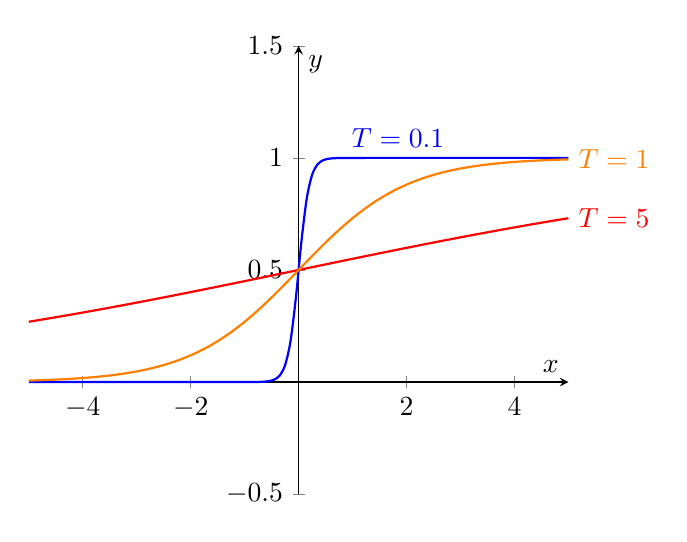
\begin{tikzpicture}
\begin{axis}[
	axis lines = middle,
	xlabel = $x$,
	ylabel = $y$,
	ymin = -0.5,
	ymax = 1.5,
	xmin = -5,
	xmax = 5,
	clip = false,
]
\addplot[
	samples = 100, 
	color = red,
	thick, smooth,
	]
{1/(1+e^(-x/5))}
node[right,pos=1] {$T=5$};
\addplot[
	samples = 100, 
	color = blue,
	thick, smooth,
	]
{1/(1+e^(-x/0.1))}
node[above,pos=0.7] {$T=0.1$};

\addplot[
	samples = 100, 
	color = orange,
	thick, smooth,
	]
{1/(1+e^(-x))}
node[right,pos=1] {$T=1$};
\end{axis}
\end{tikzpicture}
\caption{Sigmoid function (orange), with high temperature (red) and low temperature (blue).}
\label{fig:bm-simulated-annealing}
\end{figure}

\subsection{Why to restrict BMs}
Unrestricted Boltzmann machines are very powerful and can compute every function. But due the complex net structure the training is very slow and computational expensive.


